\documentclass{compiladores}
\usepackage{subcaption}

\usepackage{tikz}
\usepackage{qtree}
\usetikzlibrary{shadows,trees}
\usetikzlibrary{positioning,shadows,arrows,trees,shapes,fit}
\usetikzlibrary{graphs}

\renewcommand{\flecha}{$\rightarrow$}
\newcommand{\vazio}{{\LARGE$\epsilon$}\xspace}

\begin{document}

\begin{center}
{\LARGE Material de Apoio \#70} \\
{\bf Esquemas de tradução para expressões lógicas por controle de fluxo}
\end{center}

\section{Esquemas de tradução}

Para o {\bf and} lógico, temos o esquema de tradução.

\begin{tabular}{lll}
  B & \flecha & \{ \et{B$_1$.f = B.f; B$_1$.t = rot();} \} B$_1$ \\
    &         & {\bf and} \\
    &         & \{ \et{B$_2$.f = B.f; B$_2$.t = B.t;} \} B$_2$ \{ \et{B.code = B$_1$.code || ``B$_1$.t:'' ||  B$_2$.code;} \} \\
\end{tabular}

Para o {\bf or} lógico, temos:

\begin{tabular}{lll}
  B & \flecha & \{ \et{B$_1$.f = rot(); B$_1$.t = B.t;} \} B$_1$ \\
    &         & {\bf or} \\
    &         & \{ \et{B$_2$.f = B.f; B$_2$.t = B.t;} \} B$_2$ \{ \et{B.code = B$_1$.code || ``B$_1$.f:'' ||  B$_2$.code;} \} \\
\end{tabular}

As diferenças entre o {\bf and} e o {\bf or} lógicos são pequenas, mas
fundamentais: elas aparecem no parâmetros para o primeiro termo da
expressão (B$_1$) e também no rótulo da sintetização de código. Por
fim, a expressão relacional:

\begin{tabular}{lll}
  B & \flecha & E$_1$ {\bf op} E$_2$ \\
    &         &  \{ \et{B.code = E$_1$.code ||
    E$_2$.code || ``cmp E$_1$.temp, E$_2$.temp -> cc'' ||
    ``cbr\_LT cc -> B.t, B.f''}; \} \\
\end{tabular}

\section{Um exemplo de uso}

Considerando a seguinte expressão lógica: $a<b \lor c<d \land e<f$,
qual o código gerado a partir do esquema de tradução. Suponha que as
variáveis já estão em registradores e que o B raiz tem os sequintes
atributos herdados já definidos: \et{B.t = L0; B.f = L1;}. Veja a
solução final nas figuras~\ref{70-fig1} e~\ref{70-fig2}.

\begin{figure}[!htb]
  \centering
  \begin{subfigure}[b]{.57\textwidth}
    \centering
    \includegraphics[width=\linewidth]{img/70-1.jpg}
    \caption{Principal.}
    \label{70-fig1}
  \end{subfigure}
  ~
  \begin{subfigure}[b]{.4\textwidth}
    \centering
    \includegraphics[width=\linewidth]{img/70-2.jpg}
    \caption{Auxiliar.}
    \label{70-fig2}
  \end{subfigure}
  \caption{Solução do exemplo de uso.}
\end{figure}



\end{document}


O algoritmo de subconjuntos é responsável pela conversão de um
autômato finito \emph{não-determinístico} para o autômato
\emph{determinístico} correspondente. Esse algoritmo é fundamental na
geração automática de código de reconhecimento de analisadores
léxicos, nas situações onde expressões regulares são definidas pelo
projetista para descrever os \emph{tokens} da linguagem a ser
implementada no compilador. As expressões regulares são transformadas
através da {\bf Construção de Thompson} em autômatos finitos
não-determinísticos que são por sua vez convertidos em autômatos
finitos determinísticos através do algoritmo de subconjuntos.

\section{Preliminares}

Um autômato finito não-determinístico se defina por ter pelo
menos uma destas duas características:
\begin{itemize}
\item Tem pelo menos uma transição vazia (\vazio) entre dois
  estados \\
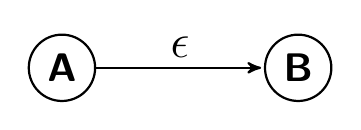
\begin{tikzpicture}[->,>=stealth',shorten >=1pt,auto,node distance=3cm,  thick,main  node/.style={circle,fill=white,draw,font=\sffamily\Large\bfseries}]
\node[main node] (1) {A};
  \node[main node] (2) [right of=1] {B};
  \path[every node/.style={font=\sffamily\small}]
    (1) edge node [bend right] {\vazio} (2);
\end{tikzpicture}


\item Ter mais de uma transição com o mesmo símbolo a partir de um
  mesmo estado \\
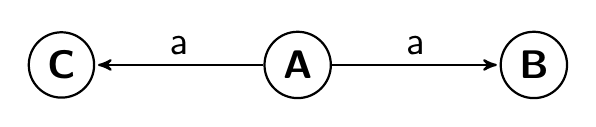
\begin{tikzpicture}[->,>=stealth',shorten >=1pt,auto,node distance=3cm,  thick,main  node/.style={circle,fill=white,draw,font=\sffamily\Large\bfseries}]
  \node[main node] (1) {A};
  \node[main node] (2) [right of=1] {B};
  \node[main node] (3) [left of=1] {C};
  \path[every node/.style={font=\sffamily\small}]
    (1) edge node [bend right] {\Large a} (2);
  \path[every node/.style={font=\sffamily\small}]
    (1) edge node [bend left, above] {\Large a} (3);
\end{tikzpicture}
\end{itemize}

No primeiro ponto, a transição vazia (\vazio) implica que uma vez no
estado de origem, não sabe-se de forma determínistica se devemos não
consumir a entrada realizando portanto a transição vazia, ou adotar
outra transição no autômato com consumo da entrada. No segundo ponto,
não há uma forma direta de decidir se devemos realizar a transição do
estado central (A) para (B) consumindo $a$ ou ir para o outro estado
(C) consumindo esse mesmo símbolo. Estamos portanto com situações
não-determinísticas. Na prática, isso implica que existem múltiplas, e
possivelmente infinitas, formas de se reconhecer uma determinada
entrada válida de um autômato não-determinista. Este fato complica a
implementação desse tipo de autômato em um programa de computador.

\section{Visão geral}

Considerando um autômato finito \emph{não-determinístico} $N$ e um
autômato finito \emph{determinístico} $D$, a visão geral que inspira o
algoritmo de subconjuntos é que cada estado no autômato determinista
equivale a um conjunto de estados do autômato não-determinista. A
ideia do algoritmo é portanto detectar quais são estes (sub)conjuntos de
estados. Essa detecção é feita através de duas operações fundamentais:
o fechamento vazio (Fechamento-\vazio) e o movimento.

\section{Operações}

Existem duas operações fundamentais no algoritmo de subconjuntos:
Fechamento-\vazio e Movimento. Os exemplos abaixo são realizados sobre
o autômato finito não-determinístico ilustrando no diagrama de
transição da Figura~\ref{afnd}.


\begin{figure}[!htb]
\centering
\resizebox{.7\linewidth}{!}{
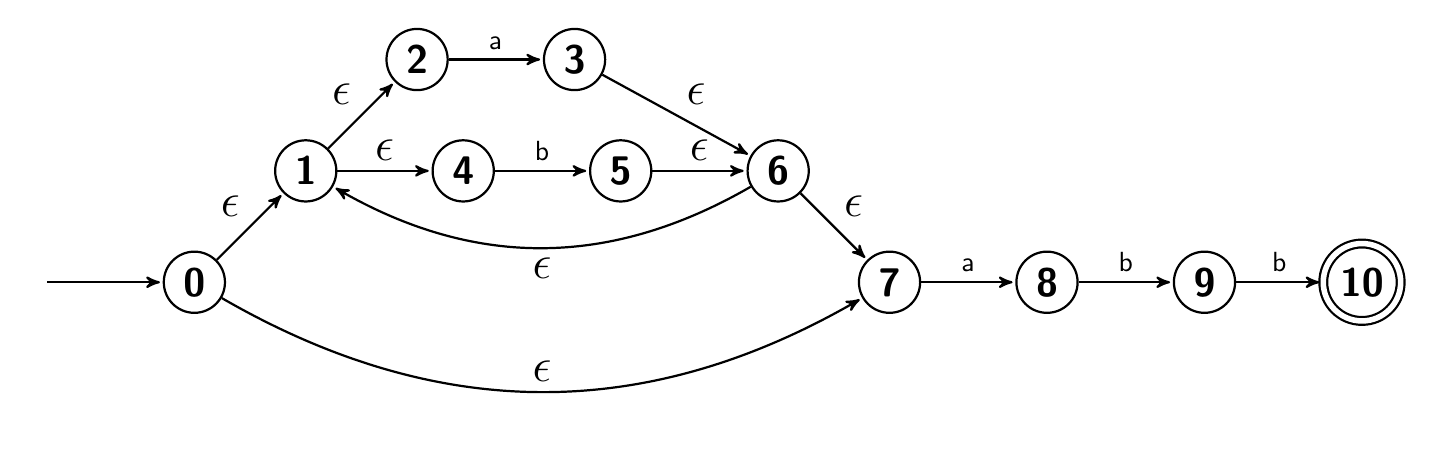
\begin{tikzpicture}[->,>=stealth',shorten >=1pt,auto,node
  distance=2cm,double
  distance=2pt,thick,main/.style={circle,fill=white,draw,font=\sffamily\Large\bfseries}]
  \node[main] (0)  {0};
  \node (A) [left of=0]  {};
  \node[main] (1) [above right of=0] {1};
  \node[main] (2) [above right of=1] {2};
  \node[main] (3) [right of=2] {3};
  \node[main] (4) [right of=1] {4};
  \node[main] (5) [right of=4] {5};
  \node[main] (6) [right of=5] {6};
  \node[main] (7) [below right of=6] {7};
  \node[main] (8) [right of=7] {8};
  \node[main] (9) [right of=8] {9};
  \node[main] (10) [right of=9, double] {10};
  \path[every node/.style={font=\sffamily}]
     (A) edge node {} (0)
     (0) edge node { \vazio } (1)
     (0) edge [bend right] node { \vazio } (7)
     (1) edge node { \vazio } (2)
     (2) edge node { a }      (3)
     (1) edge node { \vazio } (4)
     (4) edge node { b }      (5)
     (5) edge node { \vazio } (6)
     (3) edge node { \vazio } (6)
     (6) edge node { \vazio } (7)
     (6) edge [bend left] node { \vazio } (1)
     (7) edge node { a      } (8)
     (8) edge node { b      } (9)
     (9) edge node { b      } (10);
\end{tikzpicture}}
\caption{Autômato finito não-determinístico para a expressão $(a|b)^{*}abb$}
\label{afnd}
\end{figure}

\subsection{Fechamento-\vazio}

O Fechamento-\vazio ({\bf e}) é definido como o conjunto de estados
alcançados a partir do estado {\bf e} utilizando única e
exclusivamente transições vazias e incluem por definição e próprio
estado {\bf e}. Considerando o autômato não-determinístico
$(a|b)^{*}abb$ ilustrado na Figura~\ref{afnd}, o Fechamento-\vazio(1)
é o subconjunto de estados \{ 1, 2, 4 \}, onde o estado 1 é adicionado
por definição e os outros dois estados são adicionados ao subconjunto
pois é possível atingí-los somente com transições vazias diretas a
partir do estado 1. O Fechamento-\vazio(5) é o subconjunto de estados
\{ 5, 6, 7, 1, 2 e 4 \}. O estado 5 é adicionado pela definição do
fechamento, enquanto que os estados 6, 7, 1, 2 e 4 são atingidos
unicamente por transições vazias (observe o autômato da
Figura~\ref{afnd}).

O Fechamento-\vazio pode também ser calculado a partir de um conjunto
de estados. Por exemplo, podemos querer calcular o
Fechamento-\vazio(\{ 3, 5 \}). Neste caso, simplesmente calculamos o
Fechamento-\vazio(3) e realizamos a união deste resultado com o obtido
do Fechamento-\vazio(5). Sendo assim, temos:

\begin{center}
Fechamento-\vazio(\{ 3, 5 \}) = Fechamento-\vazio(3) $\cup$ Fechamento-\vazio(5)
\end{center}

O fechamento de um subconjunto de estados é necessário para a operação de
Movimento, descrita a seguir.

\subsection{Movimento}

A operação de Movimento é utilizada para calcular uma transição a
partir de um determinado estado e utilizando um determinado símbolo da
gramática. Portanto, denota-se Movimento({\bf e}, {\bf s}). O
movimento neste caso, caracteriza-se pelo conjunto de estados
alcançados a partir do estado {\bf e} do autômato consumindo
unicamente o símbolo {\bf s} através de uma única transição. Sempre,
imediatamente após o cálculo do Movimento, realiza-se o
Fechamento-\vazio do conjunto resultante.  Considerando o autômato da
Figura~\ref{afnd}, o Movimento(2, a) é \{ 3 \}, mas calculando-se o
fechamento do resultado, portanto de Fechamento-\vazio(\{ 3 \}),
obtemos o conjunto resultante do movimento \{ 3, 6, 1, 2, 4, 7 \},
pois a partir do estado 2 atinge-se o estado 3 consumindo apenas o
símbolo a; os demais estados são calculados realizando-se o fechamento
do estado 3. A operação de movimento é portanto descrita como
Fechamento-\vazio(Movimento ({\bf e}, {\bf s})).

Da mesma forma que no fechamento, a operação de movimento pode ser
calculada a partir de um conjunto de estados. Sobre o exemplo da
Figura~\ref{afnd}, o Fechamento-\vazio (Movimento (\{ 2, 7 \}, a)) é
definido como \{ 3, 8 \} pois há uma transição direta entre os estados
2 e 3 com o símbolo a; e entre 7 e 8 com o mesmo símbolo. Realizando o
Fechamento-\vazio deste resultado, obtemos o conjunto final \{ 3, 8,
6, 1, 2, 4, 7 \}.

\section{Funcionamento}

O algoritmo de subconjuntos inicia-se pelo cálculo do
Fechamento-\vazio do estado inicial do autômato finito.
não-determinístico. O próximo passo é calcular o fechamento do
movimento do conjunto de estados obtidos considerando cada um dos
símbolos pertecentes a linguagem. O processo se repete iterativamente
até todos os subconjuntos terem sido tratados e quando nenhum novo
subconjunto é criado. Dois subconjuntos são diferentes se a quantidade
de estados difere ou se há pelo menos um estado presente em um e não
no outro. Os diferentes subconjuntos de estados representam os novos
estados do autômato finito \emph{determinístico} correspondente, e os
movimentos com os diferentes símbolos da linguagem configuram as
transições entre estes estados. O estado inicial do novo autômato
determinístico é aquele que representa o fechamento-\vazio do estado
inicial do autômato não-determinístico. Os estados finais do
determinista são todos aqueles que tem em seus respectivos
subconjuntos pelo menos um estado final do autômato não-determinista
de origem.

\section{Exemplo baseado na Figura~\ref{afnd}}

O autômato da Figura~\ref{afnd} é \emph{não-determinista} pois existem
transições com \vazio. Ele tem 11 estados: de 0 a 10; e dois símbolos
pertencentes a gramática: {\bf a} e {\bf b}. Vamos convertê-lo para o
autômato determinista correspondente. Iniciamos através do cálculo do Fechamento-\vazio do estado 0 (estado inicial):

\begin{itemize}
\item Fechamento-\vazio(\{ 0 \}) = \{ 0, 1, 2, 4, 7 \}
\end{itemize}

Como o subconjunto é original \{ 0, 1, 2, 4, 7 \}, vamos nomeá-lo
subconjunto {\bf A}. O próximo passo é calcular o fechamento do
movimento do subconjunto A acima com os dois símbolos da linguagem:

\begin{itemize}
\item Fechamento-\vazio(Movimento(A, {\bf a})) = \{ 3, 8, 6, 1, 2, 4, 7 \} 
\item Fechamento-\vazio(Movimento(A, {\bf b})) = \{ 5, 6, 1, 2, 4, 7 \}
\end{itemize}

Acabamos de criar dois novos subconjuntos originais, pois são
diferentes do subconjunto A já existente. Nomeamos o subconjunto \{ 3,
8, 6, 1, 2, 4, 7 \} como subconjunto {\bf B} e o subconjunto \{ 5, 6,
1, 2, 4, 7 \} como {\bf C}. O próximo passo é realizar o fechamento do
movimento com os símbolos a partir destes dois novos
subconjuntos. Começamos pelo subconjunto B:

\begin{itemize}
\item Fechamento-\vazio(Movimento(B, {\bf a})) = \{ 3, 8, 6, 1, 2, 4, 7 \}
(subconjunto já existe, é o próprio {\bf B})
\item Fechamento-\vazio(Movimento(B, {\bf b})) = \{ 9, 5, 6, 1, 2, 4, 7 \} 
\end{itemize}

O subconjunto \{ 3, 8, 6, 1, 2, 4, 7 \} já existe e é o {\bf B}, mas o
subconjunto \{ 9, 5, 6, 1, 2, 4, 7 \} criado da transição de {\bf B}
com {\bf b} é um original que nomeamos de subconjunto {\bf D}.
%
Já tratamos neste ponto os movimentos a partir dos subconjuntos A e B,
devemos agora tratar os subconjuntos C e D. Começando por C, temos:

\begin{itemize}
\item Fechamento-\vazio(Movimento(C, {\bf a})) = \{ 8, 3, 6, 1, 2, 4, 7 \} (que é o subconjunto B) 
\item Fechamento-\vazio(Movimento(C, {\bf b})) = \{ 5, 6, 1, 2, 4, 7 \} (que é o próprio subconjunto C) 
\end{itemize}

Em seguida, tratamos os movimentos a partir do subconjunto D:

\begin{itemize}
\item Fechamento-\vazio(Movimento(D, {\bf a})) = \{ 3, 8, 6, 1, 2, 4, 7 \} (que é o subconjunto B) 
\item Fechamento-\vazio(Movimento(D, {\bf b})) = \{ 10, 5, 6, 1, 2, 4, 7 \}
\end{itemize}

O subconjunto \{ 10, 5, 6, 1, 2, 4, 7 \} configura um novo estado {\bf
  E} que é final pois ele tem o estado 10 do autômato de
origem. Embora já tenhamos detectado que o subconjunto E é final,
devemos ainda assim calcular o fechamento do movimento a partir deste
novo estado pois sempre há a possibilidade de se criar novos
estados. Então temos:

\begin{itemize}
\item Fechamento-\vazio(Movimento(E, {\bf a})) = \{ 3, 8, 6, 1, 2, 4, 7 \} (B) 
\item Fechamento-\vazio(Movimento(E, {\bf b})) = \{ 5, 6, 1, 2, 4, 7 \} (C)
\end{itemize}

A Tabela~\ref{tabela} resume as informações. 
Podemos representar através de uma diagrama de transições as
informações da Tabela~\ref{tabela}, criando o autômato determinista
correspondete. A Figura~\ref{afd} ilustra esse novo autômato.

\begin{table}[!htb]
\begin{center}
\caption{Resumo das transições da conversão do autômato da
  Figura~\ref{afnd}}
\label{tabela}
\begin{tabular}{lcccl}\toprule
            &               & \multicolumn{2}{c}{\bf Transições} \\
{\bf Subconjunto} & {\bf Identificador} & {\bf a} & {\bf b} & {\bf Comentário}\\\toprule
 \{ 0, 1, 2, 4, 7 \}       & A & B & C & Calculado a partir do Fechamento-\vazio(0) \\\midrule
\{ 3, 8, 6, 1, 2, 4, 7 \}  & B & B & D & \\\midrule
\{ 5, 6, 1, 2, 4, 7 \}     & C & B & C & \\\midrule
\{ 9, 5, 6, 1, 2, 4, 7 \}  & D & B & E & \\\midrule
\{ 10, 5, 6, 1, 2, 4, 7 \} & E & B & C & Estado E é final pois tem 10 \\\bottomrule
\end{tabular}
\end{center}
\end{table}


\begin{figure}[!htb]
\centering
\resizebox{.29\linewidth}{!}{
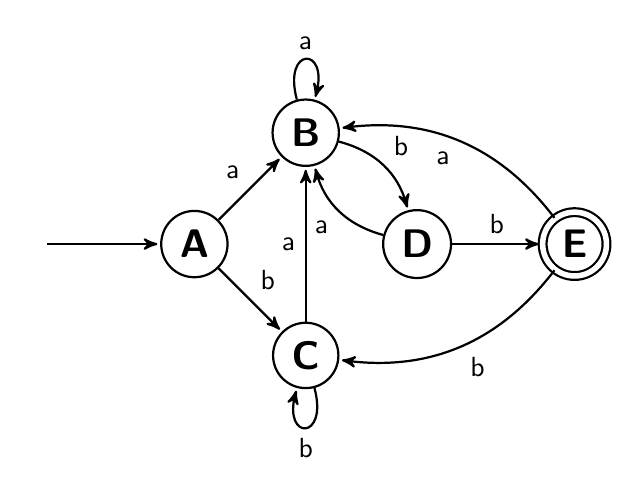
\begin{tikzpicture}[->,>=stealth',shorten >=1pt,auto,node
  distance=2cm,double
  distance=2pt,thick,main/.style={circle,fill=white,draw,font=\sffamily\Large\bfseries}]
  \node[main] (A)  {A};
  \node (Z) [left of=A]  {};
  \node[main] (B) [above right of=A] {B};
  \node[main] (C) [below right of=A] {C};
  \node[main] (D) [below right of=B] {D};
  \node[main] (E) [right of=D, double] {E};
  \path[every node/.style={font=\sffamily}]
     (Z) edge node {} (A)
     (A) edge node { a } (B)
     (A) edge node { b } (C)
     (B) edge [loop above] node { a } ()
     (B) edge [bend left] node { b } (D)
     (C) edge node { a } (B)
     (C) edge [loop below] node { b } ()
     (D) edge [bend left] node { a } (B)
     (D) edge node { b } (E)
     (E) edge [bend right] node { a } (B)
     (E) edge [bend left] node { b } (C);

     % (0) edge [bend right] node { \vazio } (7)
     % (1) edge node { \vazio } (2)
     % (2) edge node { a }      (3)
     % (1) edge node { \vazio } (4)
     % (4) edge node { b }      (5)
     % (5) edge node { \vazio } (6)
     % (3) edge node { \vazio } (6)
     % (6) edge node { \vazio } (7)
     % (6) edge [bend left] node { \vazio } (1)
     % (7) edge node { a      } (8)
     % (8) edge node { b      } (9)
     % (9) edge node { b      } (10);
\end{tikzpicture}}
\caption{Autômato finito determinístico para a expressão $(a|b)^{*}abb$}
\label{afd}
\end{figure}


\end{document}